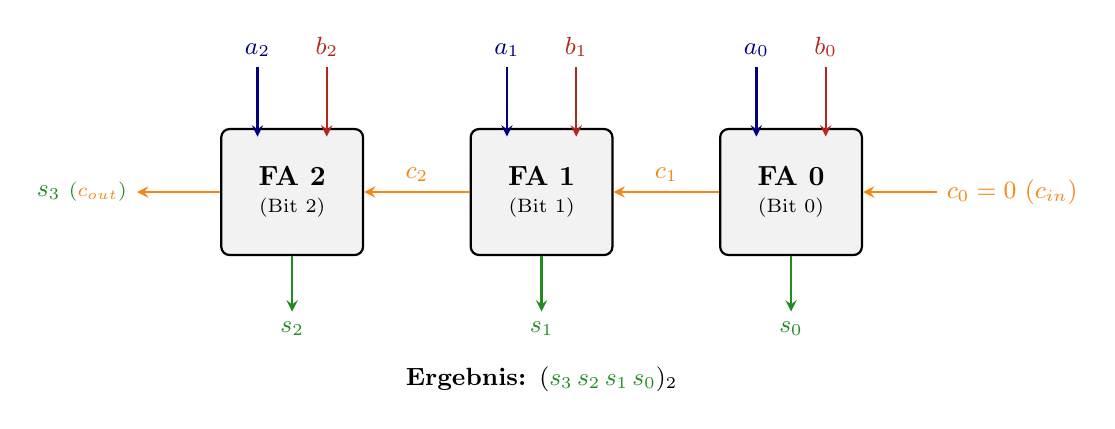
\begin{tikzpicture}[
    scale=0.88, >=stealth,
    fa/.style={draw, thick, fill=gray!10, rounded corners=3pt, minimum width=1.8cm, minimum height=1.6cm, align=center},
    wire/.style={thick, ->}
]
    % FA Blocks (Bit 2 on left, Bit 0 on right)
    \node[fa] (fa2) at (0, 0) {\textbf{FA 2}\\[-2pt]{\scriptsize (Bit 2)}};
    \node[fa] (fa1) at (3.6, 0) {\textbf{FA 1}\\[-2pt]{\scriptsize (Bit 1)}};
    \node[fa] (fa0) at (7.2, 0) {\textbf{FA 0}\\[-2pt]{\scriptsize (Bit 0)}};

    % Inputs from top (a_i in NavyBlue, b_i in BrickRed)
    \draw[wire, NavyBlue] (-0.5, 1.8) node[above, font=\small, NavyBlue] {$a_2$} -- (-0.5, 0.8);
    \draw[wire, BrickRed] (0.5, 1.8) node[above, font=\small, BrickRed] {$b_2$} -- (0.5, 0.8);

    \draw[wire, NavyBlue] (3.1, 1.8) node[above, font=\small, NavyBlue] {$a_1$} -- (3.1, 0.8);
    \draw[wire, BrickRed] (4.1, 1.8) node[above, font=\small, BrickRed] {$b_1$} -- (4.1, 0.8);

    \draw[wire, NavyBlue] (6.7, 1.8) node[above, font=\small, NavyBlue] {$a_0$} -- (6.7, 0.8);
    \draw[wire, BrickRed] (7.7, 1.8) node[above, font=\small, BrickRed] {$b_0$} -- (7.7, 0.8);

    % Carry chain in BurntOrange (from right to left)
    \draw[wire, BurntOrange] (9.3, 0) node[right, font=\small, BurntOrange] {$c_0 = 0$ ($c_{\text{in}}$)} -- (fa0.east);
    \draw[wire, BurntOrange] (fa0.west) -- node[above, font=\small, BurntOrange] {$c_1$} (fa1.east);
    \draw[wire, BurntOrange] (fa1.west) -- node[above, font=\small, BurntOrange] {$c_2$} (fa2.east);
    \draw[wire, BurntOrange] (fa2.west) -- ++(-1.2, 0) node[left, font=\small, ForestGreen] {\textbf{$s_3$} {\scriptsize (\textcolor{BurntOrange}{$c_{\text{out}}$})}};

    % Sum outputs in ForestGreen (to bottom)
    \draw[wire, ForestGreen] (fa2.south) -- ++(0, -0.8) node[below, font=\small, ForestGreen] {\textbf{$s_2$}};
    \draw[wire, ForestGreen] (fa1.south) -- ++(0, -0.8) node[below, font=\small, ForestGreen] {\textbf{$s_1$}};
    \draw[wire, ForestGreen] (fa0.south) -- ++(0, -0.8) node[below, font=\small, ForestGreen] {\textbf{$s_0$}};

    % Summary label
    \node[font=\small\bfseries, align=center] at (3.6, -2.7) {Ergebnis: $(\textcolor{ForestGreen}{s_3 \, s_2 \, s_1 \, s_0})_2$};
\end{tikzpicture}
